\documentclass{acm_proc_article-sp}

\usepackage[T1]{fontenc}
\usepackage{polyglossia}
\setdefaultlanguage{english}
\usepackage{csquotes}

\usepackage{fontspec}
\usepackage{xltxtra}
\usepackage{libertine}

\usepackage[usenames, dvipsnames]{xcolor}
\graphicspath{{./img/}}

\usepackage[backend=biber, style=numeric]{biblatex}\bibliography{literatur.bib}

\usepackage{subcaption}
\usepackage{fancyref}

\usepackage[%
unicode=true,%
colorlinks=true,%
linkcolor=black,%
urlcolor=MidnightBlue,%
citecolor=black,%
filecolor=black%
]
{hyperref}


\newcommand{\todo}[1]{\textcolor{Red}{#1}}
\newcommand{\sebastian}[1]{\textcolor{Green}{#1}}
\newcommand{\stefan}[1]{\textcolor{BurntOrange}{#1}}
\newcommand{\etal}{\textit{et. al.}}
\newcommand{\Gray}[1]{\textcolor{Gray}{#1}}

\begin{document}

\title{
Interactive Simulation WS 15/16\\ %
Project Report
}
\subtitle{EYES - Exchange Your Vision Simulator}
\numberofauthors{2}
\author{
% 1st. author
\alignauthor
Sebastian Lemp\\
%       \affaddr{Street, House}\\
%       \affaddr{PLZ City}\\
%       \affaddr{Country}\\
%       \email{sebastian.lemp@student.uni-augsburg.de}
% 2nd. author
\alignauthor
Stefan Büttner\\
%       \affaddr{Street, House}\\
%       \affaddr{PLZ City}\\
%       \affaddr{Country}\\
%       \email{stefan.buettner@student.uni-augsburg.de}
}
%\additionalauthors{Additional Authors}

% The date is actually not used in the acm template
\date{University of Augsburg, \today}

% Not neede for our purposes
%\terms{Terms}
%\keywords{Keyword 1, Keyword 2}
%% A category with the (minimum) three required fields
%\category{H.4}{Information Systems Applications}{Miscellaneous}
%%A category including the fourth, optional field follows...
%\category{D.2.8}{Software Engineering}{Metrics}[complexity measures, performance measures]

%% For the ACM ToG format
%\acmformat{ACMFormat}
%\acmVolume{Vol.}
%\acmNumber{Nr.}
%\acmYear{YYYY}
%\acmMonth{MM}
%\acmArticleNum{XXX}
%\doi{DOI}


\maketitle
\begin{abstract}
    \todo{write abstract}
    Many diseases can be treated well if recognized early, that's why we want to inform the users about different eye diseases and their effects on the vision.
\end{abstract}

% Disease list:
% -------------------------------------------------------------------------------
% (Stefan)     11 Disorders of sclera, cornea, iris and ciliary body
% (Sebastian)   1 Cataract (Grauer Star)
% (Stefan)      2 Retinal detachment and breaks
% (Sebastian)  14 Other retinal disorders
% (Stefan)      1 Glaucoma (Grüner Star)
% (Stefan)      2 Disorders of optic nerve and visual pathways
% (Sebastian)  10 Disorders of ocular muscles, binocular movement, accommodation and refraction
% (Stefan)      6 Visual disturbances and blindness
%              47

%
% Possible References:
% http://www.svi.cps.utexas.edu/EI466209.pdf

% http://www.icdvrat.org/2008/papers/ICDVRAT2008_S04_N06_Banks_McCrindle.pdf
%
% claim they have an real-time app for Android and iOS:
% http://www.brailleinstitute.org/sight-loss-blog/398-leading-eye-diseases.html 
%
% OpenGL real-time simulation
% http://percept.eecs.yorku.ca/papers/p127-vinnikov.pdf
% 

\section{Introduction}
Eye diseases have been an issue throughout all the human history.
In the beginning the focus layed on their treatment.
However, Virtual Reality (VR) is more and more pushing into the consumer market and could therefor be broadly used for education and thus prevention of eye diseases.
For example, the risk of suffering from retinal detachment can be greatly reduced if the signs are recognized early and a doctor is consulted.
Therefore, educational software can be used.
In addition, people would hopefully visit a doctor earlier if they already experienced a good simulation of a severe state of a disease, before they actually are in a severe state.
Other applications could be testing designs of consumer products like packaging or traffic signs or other signs at public places.

Although there are many simulations available already, they usually work on still 2D images, 2D video streams or static 3D scenes and don't have any game component.
Moreover, more sophisticated simulations are probably not easily available for public use and implementing a simulator using Unity3D in terms of an \emph{eye disease asset set} wrapped into a small game could be interesting for a broad audience.

So we implemented three visual disease simulators in Unity3D and applied them in a small game.
In this game the player has to collect items in a Supermarket, which is likely to be a well-known situation to everyone.

\section{Related Work}
There are different eye disease simulators available in the web already.
However, common ones, e.g. found on websites of health organizations, alter still 2D images and display them in the browser.
For example, the "Sehbehinderungs-Simulator" of ABSV~\cite{absv} lets the user choose from five different diseases and four different images to apply them to. 
There are also real-time simulations available as descriped by~\cite{eyediseasesim-zhuming} but the implementation is not available online.
\todo{cite this?}~\cite{eyediseasesim}

\section{Models and Methods}
%\begin{itemize}
%  \item Fulfill everyday tasks with impaired vision
%  \item Possible boni: 
%  \begin{itemize}
%    \item Get rid of disease by performing the right actions
%    e.g. take medication on the way or make a doctors appointment...
%    \item Preventive measures during the task to not get disease in next lvl
%  \end{itemize}
%  \item Target platform: Android \& Google Cardboard to address many people
%\end{itemize}

Assets: Inventory Master - uGUI (Sander Buchheim), Supermarket Interior (FireMesh), Drag and Drop Pause Menu (Cinopt Studios)

The player is able to experience different types of eye diseases varying in severity.
%This is supposed to give people better judgment on when to visit a doctor as well as the courage to do so, if they experience the symptoms of a particular disease.
%
%There will be at least the first 6 different eye diseases in \Fref{tab:eye_diseases} either to choose from in every task or appear at least once in the game.
%
%Possible tasks could be based on reading (visual acuity), distinguishing objects (color), and navigating in everyday environments (limited field of view).
%This may be realized required for cooking, working at a line in a factory sorting screws or similar things, using public transport or driving a car (at night), food shopping, going to the pharmacy getting the right medication, find hidden object given written hints, or board/care games.
The game is set in a supermarket where the player has to shop for different objects.
There are five different eye diseases to experience in five different levels.

%Ideally the chosen tasks would be individual levels which depend on each other and will tell a small story, like car driving → food shopping → cooking.
%The user can either choose the disease for the level himself or a random disease is selected in the beginning.
%The chosen disease should become worse over the time (within one level or across levels) but, if possible and accurate (neglecting the time), the user should also be able to slow down the process or even heal the disease completely.
%Therefore he/she has to take the appropriate measures for the specific disease.
%In order to convincingly convey the topic, using a VR device like the Oculus Rift or an mobile phone / Google Cardboard combination would be beneficial to the project.


As described in \cite{gazedisplays} and \cite{eyediseasesim} effects like
blurry or distorted vision, floaters, and reduced field of view can be
efficiently implemented by using fragment shaders. The individual properties
of the shaders and how to decompose the individual diseases into different
shaders (re-usability) is subject to the first research block. But since this
appears to be a very well researched topic, we're confident that we won't run
into any major difficulties.

\begin{table}
    \textbf{Glaucoma}\\
    Sudden eye pain, blurred vision and loss of vision especially in the
    outer regions.

    \vspace{1em}\textbf{Cataracts}\\
    Blurred vision especially in the center region.

    \vspace{1em}\textbf{Diabetic Retinopathy}\\
    Black spots in the view.

    \vspace{1em}\textbf{Color blindness}\\
    Some colours appear indistinguishable.

    \vspace{1em}\textbf{Achromatopsia}\\
    (Almost) No color sensitivity at all.

    \vspace{1em}\textbf{Myopia / Hyperopia}\\
    Commonly known as nearsightedness and farsightedness respectively.

    \vspace{1em}\textbf{Kreatoconus}\\
    The cornea deforms into a conical shape.
    Multiple ghost images may be visible, arranged in a chaotic pattern,
    the vision becomes blurry, and visual acuity decreases at all distances.
    Poor night vision, photo-phobia, and eye strain are additional symptoms.

    \vspace{1em}\textbf{Nyctalopia / Hermalopia}\\
    High difficulty to see in relatively low and bright light respectively.

    \vspace{1em}\textbf{Retinal detachment / Posterior vitreous detachment}\\
    Flashes of light, very brief in the extreme peripheral region.
    Sudden increase in the amount of floaters.
    Slight feeling of heaviness in the eye.
    \caption{Eye diseases}
    \label{tab:eye_diseases}
\end{table}

\section{The human eye}
In order to simulate diseased human eyes it is beneficial to know some things about it.
As can be seen in \Fref{fig:humaneye} the human eye is a spherical shaped organ.
In some aspects it can be compared to human made cameras in others they differ tremendously.

\begin{figure}
    \centering
    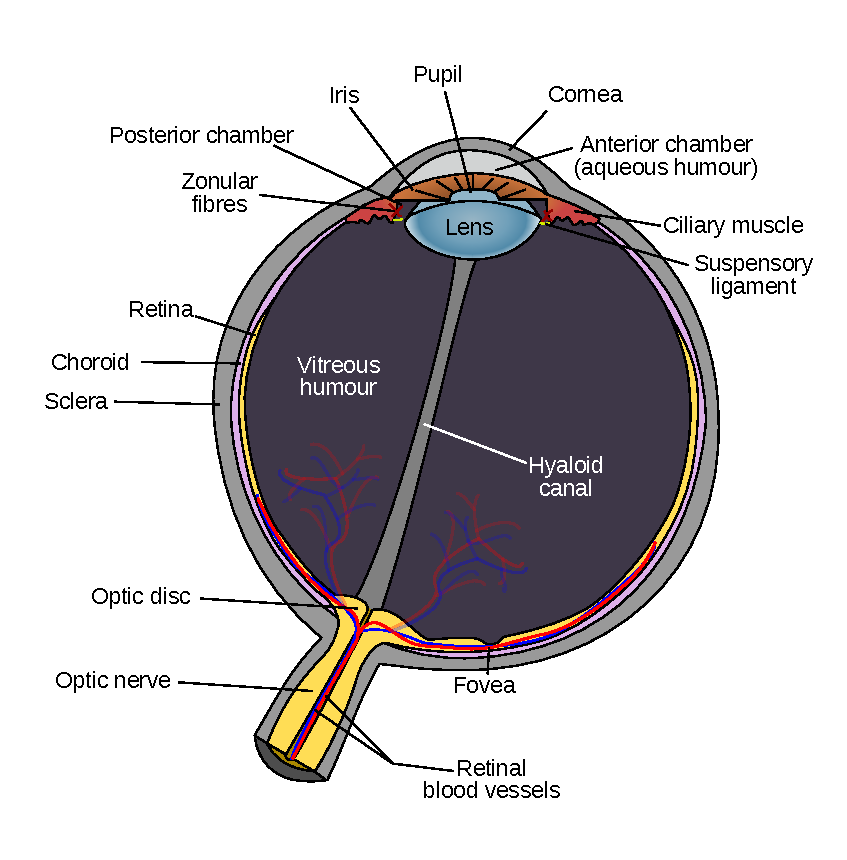
\includegraphics[width=\columnwidth]{human_eye_scheme.pdf}
    \caption{Scheme of the human eye.}
    \label{fig:humaneye}
\end{figure}

\begin{table}
    \centering
    \begin{tabular}{ll}
        Diopters                & 59-60 dpt \\
        Focal length            & 17mm/22-24mm\footnote{See \cite{eye-focal, eyeascamera}} \\
        Pupil diameter          & 2mm - 7/8mm (contracted - dilated)\footnote{See \cite{eyeascamera}} \\
        Cornea-Retina distance  & 17mm/25mm\footnote{See \cite{eyeascamera}} \\
        f-stop                  & ~f/3.2 or f/3.5\footnote{See \cite{eyeascamera}} \\
        Cone of visual attention& ~55º \\
        № Pixels                & 130 mega pix (6 mio cones, 124 rods) (compared to 24 mega pix) \\
        Macula                  & 6mm radius, 150000 px/mm²\\
        Fovea (inside macula)   & color only vision, densly packed with cones \\
    \end{tabular}
    \caption{Properties of the human eye}
    \label{tab:eyeproperties}
\end{table}

\subsection{Color blindness}
\subsection{Glaucoma}
\subsection{Myopia and Hyperopia}
\begin{description}
\item[Axial Myopia]
    Increase in the eye's axial length.\\
    Most common one!
\item[Refractive Myopia]
    \begin{description}
    \item[Curvature myopia]
    Execssive or increased curvature of one or more of the refractive surfaces of the eye. Mostly the cornea.
    \item[Index myopia]
    Variation of the index of reflection of one or more of the ocular media.
    \end{description}
\item[Nocturnal myopia]
\end{description}

For a reference on real-time focal blur/depth of field see \cite{gpugems-DoF, gpugems3-DoF}.

Change in focal length yields zoom. Big focal length = big zoom, small focal length = wide angle\\
Moving the fixed focal-length lense away and towards the canvas focuses. \\
Given the cornea-retina distance of 24mm, the focal-length range of the human eye can be estimated by [20,69mm - 24mm] for a distance range from 15cm to ∞ (see research/FocalLengthDiopters.ods) using the formula
\begin{equation}
    \frac{1}{d_p} + \frac{1}{d_I} = \frac{1}{f}.
\end{equation}
In order to simulate Myopia/Hyopia we calculate the required focal length for the altered retinal distance based on
\begin{equation}
    f = \frac{d_p d_I}{d_p + d_I}
\end{equation}
and truncate the value to the 

\section{Project Requirements}
\subsection{Science}
\subsection{Gamification}
\subsection{Complexity}
\subsection{Aesthetics}
%
%
\section{Summary \& Future Work}
Vinnikov \etal \cite{gazedisplays} developed a Gaze-Contingent-Display in order to evaluate the users eye direction and adept the displayed images in real-time.
Because the effects of eye diseases follow the eye movement, i.e. are static with respect to the eye coordinate frame, they achieved more realistic results in comparison to rendering gaze-independent images.
A consumer solution is under development by the German company SensoMotoric Instruments (SIM) which provides an gaze tracking solution update for the Oculus Rift DK 2 \cite{smi-oculus, arstechoculus}.
According to their website they also provide an integration into various VR engines, including Unity3D, available making it especially interesting for this project.

The gaze-direction would be useful to accurately simulate the vision fields and would also be an interesting human interface for the game mechanics.
%
\printbibliography

\balancecolumns

\end{document}
